\chapter{Аналитический раздел}
\label{cha:analysis}

Облака - очень сложная и выразительная часть неба. Именно облака могут создать впечатление
о надвигающихся погодных условиях.
Для создания реалистичного неба облака должны быть динамическими
и генерироваться в реальном времени. Есть множество алгоритмов для достижения этой цели.

\section{Анализ предметной области}

Рассматривая классический метод визуализации облаков с единой панорамной текстурой, Геретт предложил 
использовать технику визуального потока, чтобы создать движение в небе \cite{Gue14}. Облака будут двигаться в определенном направлении, например, ветра. Этот метод является
эффективным, однако не связан с изменением формы облаков, погоды или
освещения.

Для учета динамического освещения солнца и неба можно генерировать облака
с помощью частиц. Один из методов генерации кучевых облаков с помощью
частиц был представлен Юсовым в 2014 году \cite{hpg.20141101}.

\begin{figure}[H]
    \centering
    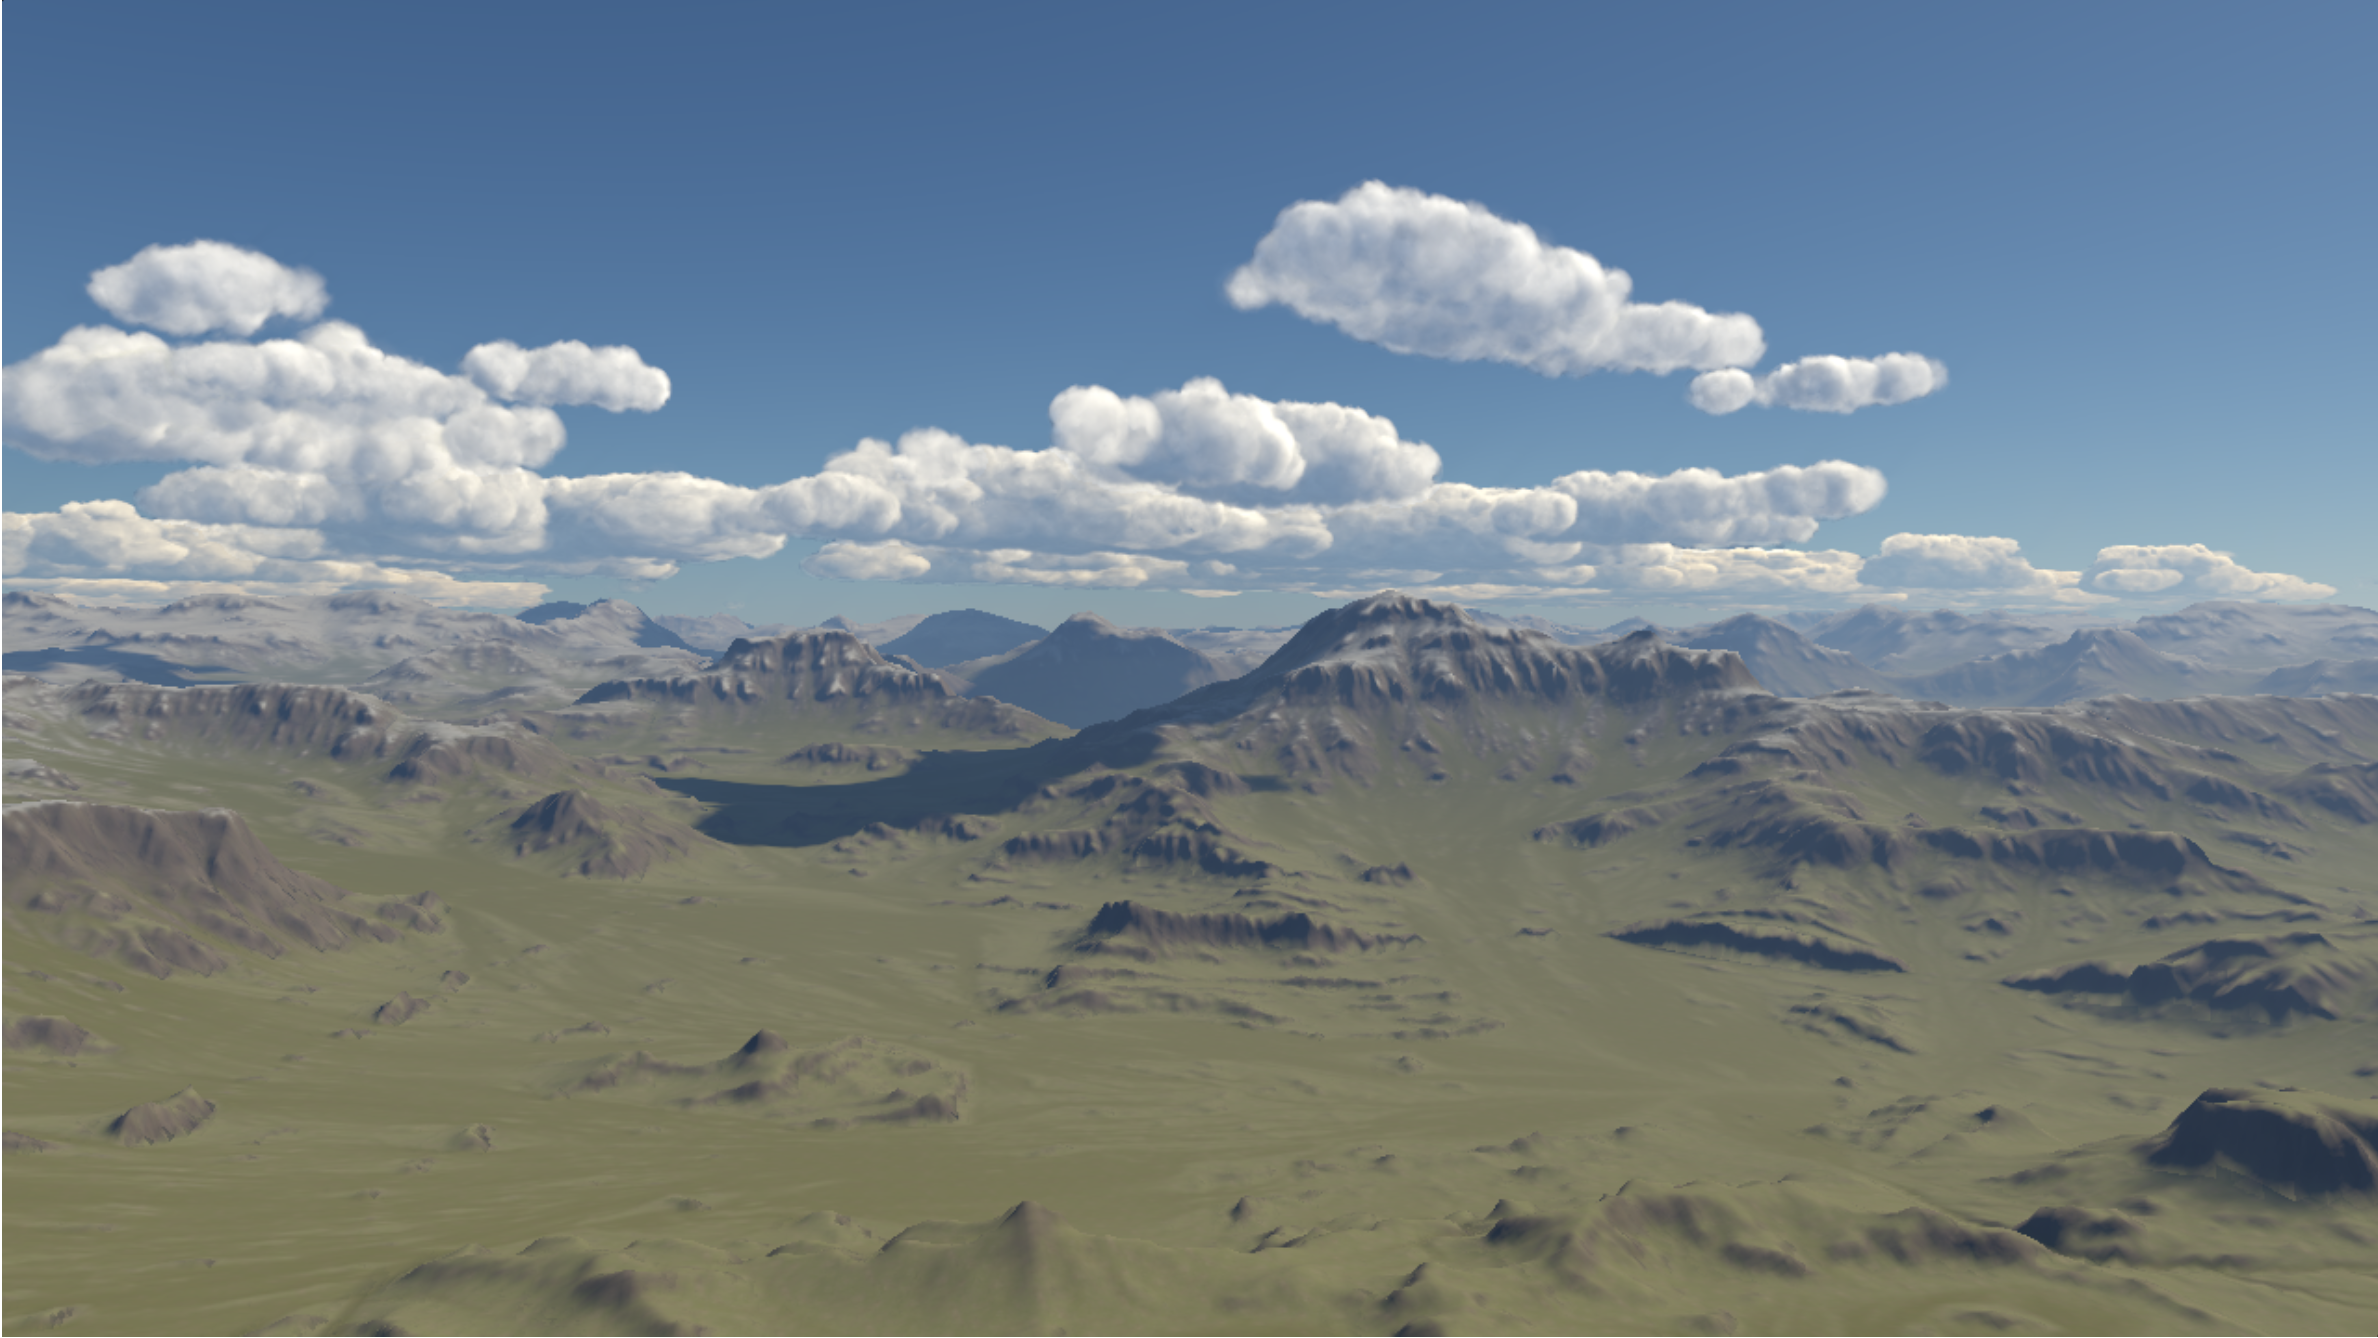
\includegraphics[scale=0.4]{img/ysov.png}
    \caption{Результат, полученный алгоритмом частиц}
    \label{img:ysov}
\end{figure}

Также для генерации кучевых облаков можно использовать алгоритм лучевого
марша, который был разобран Шнайдером \cite{Sch16}. Данный алгоритм
позволяет визуализировать динамически освещенные облака. С помощью
нескольких параметров этот метод позволяет строить сложные облачные
формы с высокой детализацией как видно на рисунке \ref{img:raymach}.
Этот метод применим к играм, в которых необходимо в реальном времени
изменять погодные условия и освещение.

\begin{figure}[H]
    \centering
    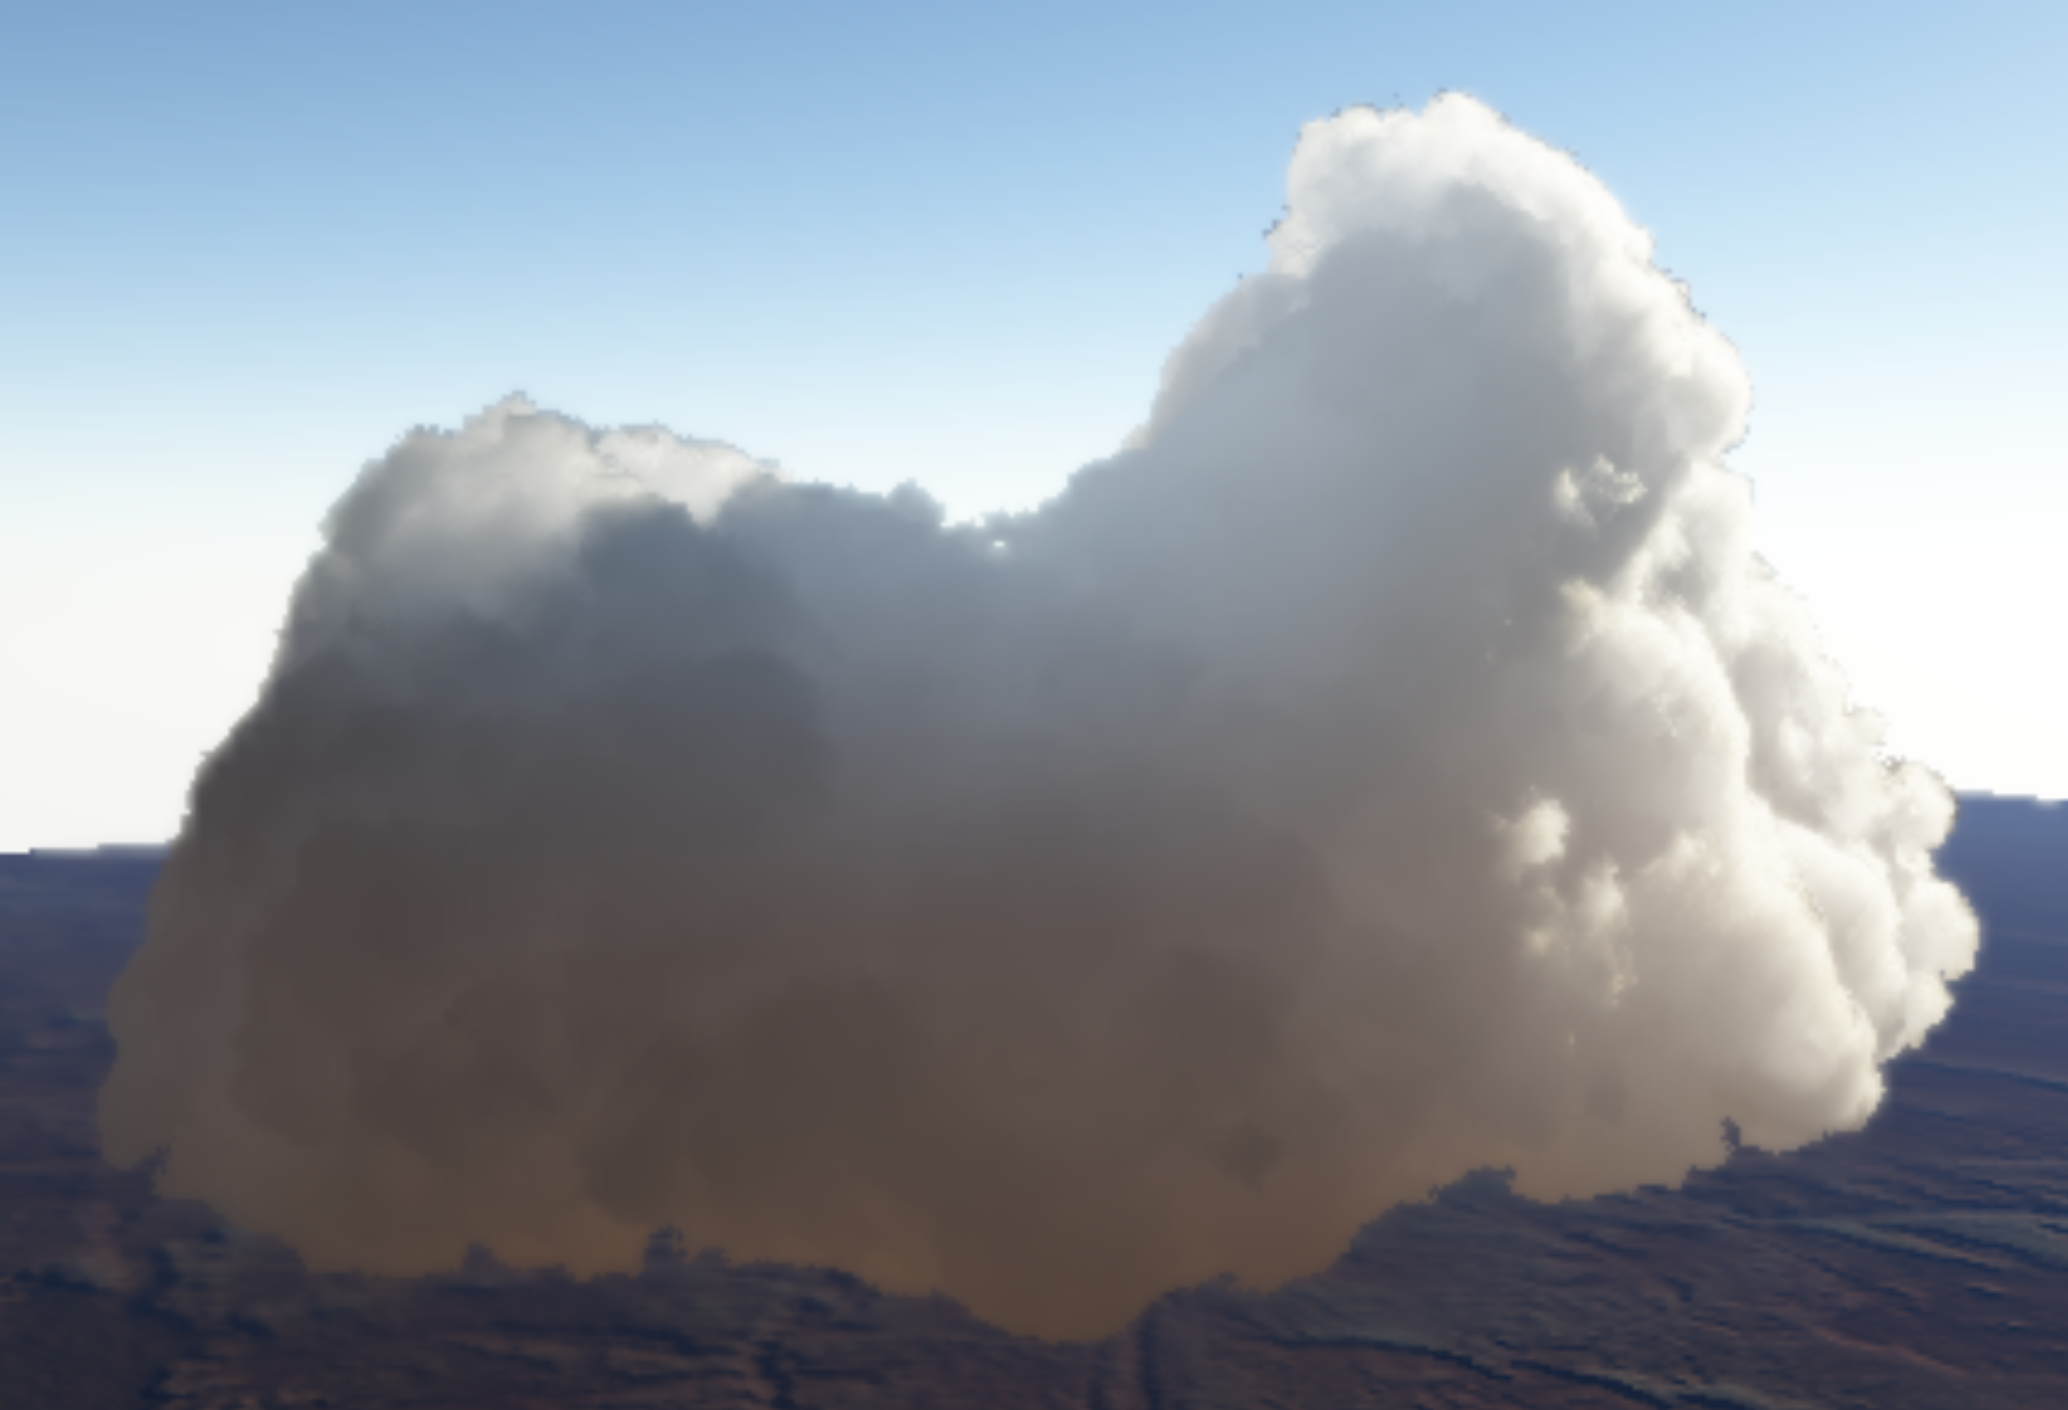
\includegraphics[scale=0.4]{img/raymach.png}
    \caption{Результат работы алгоритма лучевого марша}
    \label{img:raymach}
\end{figure}

\section{Обзор и анализ существующих программных систем и обоснование необходимости разработки}
